
\documentclass[paper-main.tex]{subfiles}


\begin{document}

% wild speculation
%We are currently working towards two improvements of the optical microphone.

The optical microphone experiment describe here can be used to convey a variety of topics as a teaching tool. 
Here we consider a selection of further extensions to the experiment touching on noise isolation, transfer function analysis, speech recognition, and control systems. 


An initial improvement is to better isolate the experiment from interference, such as the mains supply. 
The Raspberry Pi is USB powered and requires low power so it could be run off a commercial external phone battery. 
Everything else in the circuit, including the photodiode, is connected to the Pi. 
The laser is DC powered through a converter, so should not introduce mains harmonics itself. 
Transferring the circuit from a breadboard to a printed circuit board will also reduce interference~\cite{elfekey2013design}

%With the interferometer in a dark room and under a box to better isolate from any ambient light or air currents, this would hopefully remove (or better separate) all sources of the 50Hz mains hum from the optical microphone.

A second improvement is to measure the full model of the transfer function of the system. 
Theoretically, with the correct transfer function, signal recovery is limited by the signal-to-noise ratio as an optimal matched filter could be constructed.
The transfer function starts from the voltage sent to the speaker and end with the value recorded by the Pi, and include any non-linearities in the speaker audio production, the speaker-mirror coupling, the separation-intensity relation Appendix~\ref{app:intensity_derivation}, and the photodiode reading. 
A schematic of the full optical microphone transfer function is shown in Figure~\ref{fig:pipeline_highlighted}.

A voluminous literature exists about using a hidden Markov model (HMM) trained against phonemes to recognize speech~\cite{HMM_english}. 
Interestingly, this connects back to the Viterbi algorithm in Section IV, which is also underpinned by a hidden Markov model, albeit of a different type. 
Alternatively, machine learning solutions exist throughout the field that are able to compete~\cite{SEGAN} with statistical techniques like the logMMSE estimator.

Other traditional signal processing methods for extracting spectrogram like wavelet transform (WT) \citep{nason1995stationary} can also be implemented and compared with HMM. WT provides both time and frequency information, making it easier to pinpoint the origin of noise respect to time. 
In Refs. \cite{tufekci2000feature,agbinya1996discrete}, WT was also proposed for speech recognition. 

Finally, we can also consider how to improve the stability of the optical microphone components.
A feedback loop control system can be used to suppress any unwanted movement of the interferometer components~\citep{abbott2017exploring, Sekiguchi:2016bmv, verhoeven2009robust}. 

%To remove the mains hum we could also monitor it separately from the interferometer and subtract the sinusoids with the right phase and amplitude in real (not frequency) space to avoid the problems of Section~\ref{sec:simple_filters}. 
%This could be done with the existing signals if the recording duration is long enough to precisely measure the phase and amplitude over a large number of cycles.


\begin{figure*}
	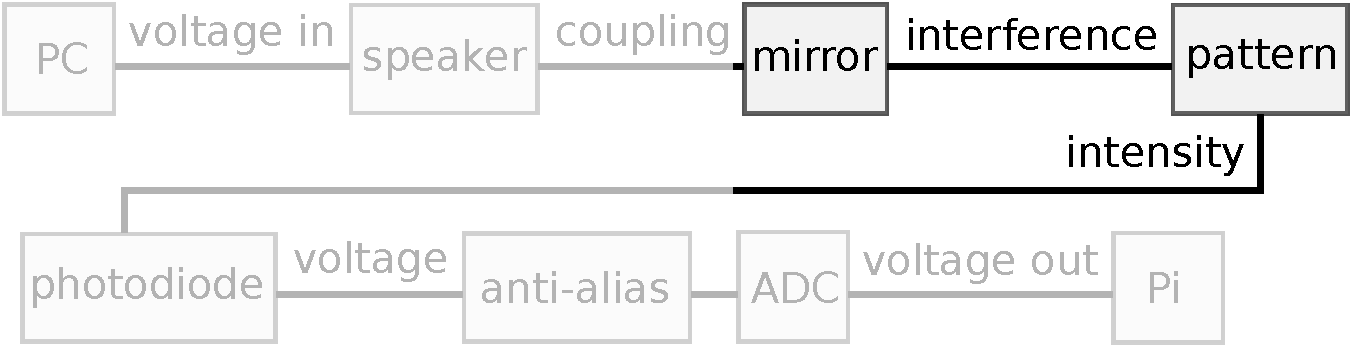
\includegraphics[width=.99\textwidth]{figures/pipeline_highlighted.pdf}
	\caption{
Flowchart for the optical microphone transfer function. 
The highlighted stage is analysised in Appendix XX, the other stages are left to future work. 
}
	\label{fig:pipeline_highlighted}
\end{figure*}

\end{document}
